%File: formatting-instruction.tex
\documentclass[letterpaper]{article}
\usepackage{aaai}
\usepackage{times}
\usepackage{helvet}
\usepackage{courier}
\usepackage{color}
\usepackage{textcomp}
\usepackage{amsthm}
\usepackage{amssymb}
\usepackage{amsmath}
\usepackage{graphicx}
\usepackage{xcolor}
\usepackage{comment}
\usepackage{xspace}
\usepackage{tikz}
\usepackage{epsdice}
\usetikzlibrary{trees}
\usetikzlibrary{shapes.geometric}

\tikzset{
  treenode/.style = {align=center, inner sep=0pt, font=\sffamily},
  ma/.style = {draw,treenode, shape border rotate=90, isosceles triangle,isosceles triangle apex angle=60, black, minimum width=2mm},% arbre rouge noir, noeud noir
  mi/.style = {ma, shape border rotate=-90},
  ch/.style = {draw, treenode, circle, minimum width=2mm, black}
}

\tikzstyle{level 1}=[level distance=8mm, sibling distance=1.5cm]
\tikzstyle{level 2}=[level distance=8mm, sibling distance=1cm]
\tikzstyle{level 3}=[level distance=8mm, sibling distance=0.5cm]

\usepackage[algo2e, noend, noline, linesnumbered]{algorithm2e}
% need these next two lines for old versions of alg2e
\providecommand{\SetAlgoLined}{\SetLine}  
\providecommand{\DontPrintSemicolon}{\dontprintsemicolon}
\DontPrintSemicolon
\makeatletter
\newcommand{\pushline}{\Indp}% Indent
\newcommand{\popline}{\Indm}
\makeatother


\newcommand{\argmin}{\operatornamewithlimits{argmin}}
\newcommand{\argmax}{\operatornamewithlimits{argmax}}
\newcommand{\bE}{\mathbb{E}}
\newcommand{\bx}{\mathbf{x}}
\newcommand{\bg}{\mathbf{g}}
\newcommand{\bu}{\mathbf{u}}
\newcommand{\bU}{\mathbf{U}}
\newcommand{\cI}{\mathcal{I}}
\newcommand{\cC}{\mathcal{C}}
\newcommand{\cP}{\mathcal{P}}
\newcommand{\cQ}{\mathcal{Q}}
\newcommand{\tta}{\mathtt{a}}
\newcommand{\tth}{\mathtt{h}}
\newcommand{\ttz}{\mathtt{z}}
\newcommand{\PW}{\mbox{PW}}
\newcommand{\BR}{\mbox{BR}}
\newcommand{\defword}[1]{\textbf{\boldmath{#1}}}
\newcommand{\ie}{{\it i.e.}\xspace}
\newcommand{\eg}{{\it e.g.}\xspace}
\newtheorem{definition}{Definition}
\newtheorem{fact}{Fact}
\newtheorem{theorem}{Theorem}
\newtheorem{corollary}{Corollary}
\newtheorem{lemma}{Lemma}
\newtheorem{proposition}{Proposition}
\newcommand{\Proof}{{\noindent\bf Proof. }}
\newcommand{\citejustyear}[1]{\cite{#1}}
\newcommand{\Qed}{$\blacksquare$}
\newcommand{\abs}[1]{\left|#1\right|}
\newcommand{\todo}[1]{{\color{red}{\bf #1}}}
\newcommand{\breturn}{{\bf return}\xspace}

% the note center!
\definecolor{darkgreen}{RGB}{0,125,0}
\newcounter{vlNoteCounter}
\newcounter{mlNoteCounter}
\newcounter{asNoteCounter}
\newcommand{\vlnote}[1]{{\scriptsize \color{blue} $\blacksquare$ \refstepcounter{vlNoteCounter}\textsf{[VL]$_{\arabic{vlNoteCounter}}$:{#1}}}}
\newcommand{\mlnote}[1]{{\scriptsize \color{darkgreen} $\blacksquare$ \refstepcounter{mlNoteCounter}\textsf{[ML]$_{\arabic{mlNoteCounter}}$:{#1}}}}
\newcommand{\asnote}[1]{{\scriptsize \color{red} $\blacktriangle$ \refstepcounter{asNoteCounter}\textsf{[AS]$_{\arabic{asNoteCounter}}$:{#1}}}}
%\newcounter{NoteCounter}
%\newcommand{\vlnote}[1]{{\scriptsize \color{blue} \refstepcounter{vlNoteCounter}\textsf{[VL]$_{\arabic{vlNoteCounter}}$:{#1}}}}
%\renewcommand{\vlnote}[1]{}

\frenchspacing
\setlength{\pdfpagewidth}{8.5in}
\setlength{\pdfpageheight}{11in}
\pdfinfo{
/Title (Searching Imperfect Information Games using Online Counterfactual Regret Minimization)
/Author (Authors)}
\setcounter{secnumdepth}{0}  
 \begin{document}
% The file aaai.sty is the style file for AAAI Press 
% proceedings, working notes, and technical reports.
%
\title{Search in Imperfect Information Games using Online\\Monte Carlo Counterfactual Regret Minimization}
\author{Authors}
%\author{Author info\\
%Association for the Advancement of Artificial Intelligence\\
%2275 East Bayshore Road, Suite 160\\
%Palo Alto, California 94303\\


\maketitle

\begin{abstract}
Online search in games has always been a core interest of artificial intelligence. 
Advances made in search for perfect information games (such as Chess, Checkers, Go, 
and Backgammon) have led to AI capable of defeating the world's top human experts. 
Search in imperfect information games (such as Poker, Bridge, and Skat) is significantly 
more challenging due to the complexities introduced by hidden information. In this 
paper, we present Online Outcome Sampling (OOS), the first imperfect information 
search algorithm that is guaranteed to converge to an equilibrium strategy in two-player 
zero-sum games. We show that OOS avoids common problems encountered by existing 
search algorithms and we experimentally evaluate its convergence rate and practical 
performance against benchmark strategies in Liar's Dice and a variant of Goofspiel. 
We show that unlike with Information Set Monte Carlo Tree Search (ISMCTS) the 
exploitability of the strategies produced by OOS decreases as the amount of search 
time increases. In practice, OOS performs as well as ISMCTS in head-to-head play 
while producing strategies with lower exploitability given the same search time.
\end{abstract}

\section{Introduction}

%Main points: 
%\begin{itemize}
%\item motivate importance of convergence to NE. 
%\item why online search vs. offline equilibrium computation
%\item existing methods may not converge over time (it would be great to have a motivating example that convinces the reader that any determinization-based II search algorithm cannot converge in general - some kind of search game could be a good example)
%\item introduce the first one that does, and show that it can compete with the others in practice
%\end{itemize}

In many sequential multi-agent interactions, agents have some initial time to prepare for the interaction and then after each decision, have  additional thinking time to decide about their next move. When preparation time is abundant and the computational resources are sufficient, an equilibrium strategy for a smaller abstract game can be pre-computed and then used during the game play. This {\it offline approach} has been remarkably successful in Computer Poker \cite{Johanson07Msc}.
However, the preparation time is often very limited. The exact model of the game may become known only shortly before acting is necessary, such as in general game-playing, security enforcement in previously unknown environment, and general-purpose robotics. In a short time, only a very small abstract game could be solved in advance. Moreover, it might not even be possible to create a sufficiently small and still useful abstraction to be solved in time. In these cases, agents may need to {\it decide online}: make initial decisions quickly and then put additional effort to improving their strategy in the current situation while the interaction is taking place.

%Search in game-playing has been a classic interest of artificial intelligence. 
%focused on perfect information games, 
When restricted to perfect information settings, the field of online search has benefited from decades of research in game-playing. 
%as evidenced by events such as defeat of human chess champions, 
%solving of checkers, and the growing strength of computer Go programs~\cite{Campbell02deepblue,Schaeffer07gameover,Gelly12}.
Due to the complexity and problems introduced by hidden information, search in imperfect information settings has received comparatively much less attention.
%This is unfortunate as many sequential decision-making problems have some element of hidden information. 
Modern approaches to imperfect information search use different forms of {\it determinization} to sample possible states, then run 
searches rooted from these states, aggregating their results to choose an action to play. The most extreme forms, \eg Perfect Information 
Monte Carlo~\cite{Long10Understanding} ``average over clairvoyance''~\cite{AIBook},
% ML-Note Nov2: @Viliam, PIMC *is* "averaging over clairvoyance"
ignoring the information structure completely. While this is sufficient in some games, it tends to have trouble in games like poker 
where information is critical. 

%; similar problems have been reported using Monte Carlo Tree Search (MCTS) in Kriegspiel~\cite{Ciancarini10Kriegspiel}.
%Most recent algorithms try to fix the problem by accounting for the information structure during the 
%search in some way. These approaches seem to improve performance in Kriegspiel, Skat~\cite{Furtak13Recursive}, 
%Scotland Yard~\cite{Nijssen12SY}, Dou Di Zhu, Magic: The Gathering, and other card games~\cite{Cowling12MTG,Cowling12ISMCTS}.

%For example, the notion of a subgame is required for backward induction, 
%which most perfect information search algorithms are based on, is not well-defined in imperfect information games. 

The main problem with current techniques is a lack of theoretical foundations of the algorithms. There are no guarantees that the algorithms will always find a good strategy in a game, given a sufficient thinking time. In fact, there is empirical evidence suggesting that some of these techniques will not converge to the optimal solution even in very small games like Biased Rock-Paper-Scissors and Kuhn poker~\cite{Shafiei09,Ponsen11Computing}.

In this paper, we start by formalizing the problem of imperfect information search from the ground up. That is, we return to the game-theoretic 
foundations upon which search in games is built to motivate the importance of Nash equilibrium as the optimal strategy in zero-sum games. We explain the subtleties introduced by imperfect information that cause the current approaches not to converge to the optimal strategy. We introduce Online Outcome Sampling (OOS), a simulation-based algorithm that builds its search tree incrementally, like MCTS.  
We show that OOS converges to an equilibrium strategy as time increases, making it the first 
known imperfect information search algorithm satisfying this property, which we call {\it consistency}. Furthermore, we analyze methods for incorporating the information obtained by the players in the game to the search process, so that the consistency property is preserved. We show the empirical convergence rates and performance of OOS, comparing them to benchmark players and to ISMCTS~\cite{Cowling12ISMCTS}, a 
recent algorithm currently used in a popular mobile phone implementation of Spades~\cite{Whitehouse13Integrating}. 

%We present results in two domains: Liar's Dice and a variant of Goofspiel.

%PIMC~\cite{Long10Understanding}, ISMCTS~\cite{Cowling12ISMCTS}, and MMCTS~\cite{Auger11Multiple}.

%\vlnote{Current intro targets particularly the search community.}

\section{Background and Related Work}

%Overview of past algorithms and the current state-of-the-art (we have to ``weave'' the related work below into a nice overview).
%Define determinization, strategy fusion, non-locality, disambiguation factor. 
%References to help:
%\begin{itemize}
%\item Original/first II search~\cite{Frank98Finding}
%\item Work on Bridge~\cite{Ginsberg01}
%\item Information Set Search~(ISS)~\cite{Parker10iss,Parker06paranoia}
%%\vlnote{\cite{Parker10iss} is a little more detailed, but I guess it is from a less reputable forum.} 
%We have used ISS in MCTS setting in a visibility-based pursuit-evasion game~\cite{Lisy12peg}
%\item Work on Hearts / Spades~\cite{Sturtevant08An}
%\item PIMC~\cite{Long10Understanding} and other work on Skat (Jeff's thesis)
%\item Counter-examples in simple games~\cite{Shafiei09,Ponsen11Computing} 
%\item MMCTS (Phantom Tic-Tac-Toe)~\cite{Auger11Multiple}
%\item Work on Exp3 for Urban rivals~\cite{Teytaud11Upper,StPierre12Online}
%\item IS-MCTS~\cite{Cowling12ISMCTS} and other work by that group (on Dou di Zhu, MTG etc. \cite{Whitehouse11DDZ,Cowling12MTG})
%\item IIMC~\cite{Furtak13Recursive}
%\item Scotland Yard~\cite{Nijssen12SY}
%\item MCTS in Kriegspiel~\cite{Ciancarini10Kriegspiel}
%\item Kurt's past work on MCTS for Poker~\cite{vdbroek09MCTSPoker}?
%%\item MCTS in Kriegspiel~\cite{Ciancarini09Kriegspiel}
%%\vlnote{why not the AIJ 2010 paper?} 
%% ML: I did not know about it.
%\item Maybe quick mention of recent excitment in simultaneous move games (SMAB, double-oracle and serialized AB algorithm that doesn't have a name, SM-MCTS, and NIPS paper
%\item Mention that OOS has been applied in SM-MCTS setting.
%\end{itemize}

% classic work: PIMC and its successes

Some of the first imperfect information search algorithms were inspired by the application to 
Bridge~\cite{Frank98Finding,Ginsberg96Partition}, and notably by the success of GIB~\cite{Ginsberg01}.
In GIB, perfect information search is performed on a {\it determinized} 
instance of the game: one where all players can see usually hidden information, a concept 
originally proposed in~\cite{Levy89Heuristic}. This approach has also performed well in other 
games like Scrabble~\cite{Sheppard02World}, Hearts~\cite{Sturtevant08An}, and Skat~\cite{Buro09Improving}. 

% overview of problems with PIMC, proposed solutions

There are several problems that have been identified with Perfect information Monte Carlo (PIMC) search techniques
on determinized samples. The most common are {\it strategy fusion} and {\it non-locality}~\cite{Frank98Finding}.
Strategy fusion occurs when an algorithm is allowed to choose two different actions from two different states in the same 
information set, which is inconsistent with the constraints imposed by the game's information structure. 
Non-locality occurs due to the assumption that subgames are well-defined and that hence search can be 
recursively applied by computing and comparing values of subgames. 

Strategy fusion can be overcome by imposing the proper information constraints during search, as was done in 
Kriegspiel~\cite{Ciancarini10Kriegspiel}, Kuhn Poker~\cite{Ponsen11Computing}, pursuit-evasion games~\cite{Lisy12peg}, 
card games and other phantom games~\cite{Cowling12ISMCTS}. 
Non-locality, however, is a fundamental problem.
Consequently, the usual minimax formulation of payoffs defined over future states is not applicable.  
The authors of \cite{Parker10iss,Parker06Overconfidence} showed that minimax-style backups at opponent information 
sets can lead to overly paranoid search. 
We also make similar observations for MCTS in Liar's Dice. 

ISMCTS is similar to MCTS except that it places a bandit at each information set rather than at each 
state~\cite{Cowling12ISMCTS}. ISMCTS builds an information set tree and aggregates utility estimates of actions 
at information sets for all determinized states among its samples. 
Consider the game in Figure~\ref{fig:coordGame}. 
Suppose a search starts from information set $I$. Because utilities for actions taken from all states are combined, 
ISMCTS will choose left and right equally as often for both players, which would correspond to the equilibrium 
strategy in the coordination subgame. However, mixing equally at is not part of an equilibrium in this game, since
it would lead to an expected utility of $\frac{3}{4}$ to the maximizing player for playing right, which 
would give incentive to the maximizer to play left more often and change the minimizer's optimal response.  

\begin{figure}
\begin{center}
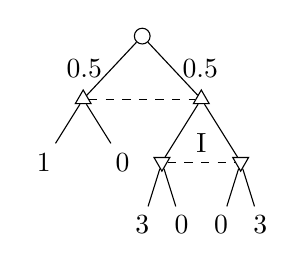
\begin{tikzpicture}
\node [ch] {}
    child{ node [ma] (i1_1) {} 
	    child{ node {1}}
    	    child{ node {0}}
    	    edge from parent node[left] {0.5}
    }
    child{ node [ma] (i1_2) {}
	    child{ node [mi] (i2_1) {}
			   child{ node {3}}
	    		   child{ node {0}}
			 }	    
	    child{ node [mi] (i2_2) {}
			   child{ node {0}}
	    		   child{ node {3}}
			 }
		edge from parent node[right] {0.5}
	};
\draw [dashed] (i1_1) -- (i1_2);
\draw [dashed] (i2_1) -- (i2_2) node[midway, above] {I};
\end{tikzpicture}
\end{center}
\caption{An example game with maximizing $\bigtriangleup$, minimizing $\bigtriangledown$ and chance $\bigcirc$ players.}\label{fig:coordGame}
\end{figure}

% other missing related works

%One particularly related work is the MMCTS algorithm~\cite{Auger11Multiple} that has been 
%applied to Phantom Tic-Tac-Toe. 
%MMCTS uses Exp3 at each information set in its search, and scales the payoff 
%received by the depth of each playout. 
%While we have not implemented MMCTS, we have been able to test our 
%algorithm against it thanks to the authors sharing their code. 

% Poker and the game-theoretic offline approach
%Billings04Game

Game-tree search techniques have also been applied to Poker~\cite{Billings04Game}. In recent years, however, 
the most common approach to producing strong Poker AI has been to use advances in equilibrium approximation 
algorithms to compute a near-optimal equilibrium of an abstract game and subsequently use the abstract strategies 
when playing the full game~\cite{Sandholm10The}. This {\it offline} approach requires designing 
abstractions and pre-computing Poker equilibria, which is often not possible. Also, due to the size of 
abstractions~\cite{Johanson13Evaluating}, the memory resources may not be available or known in advance. 

\subsection{Extensive-Form Games}

%Basic game theoretic definitions. Behavioral strategies. 
%CFR~\cite{CFR} and MCCFR~\cite{Lanctot09Sampling}. Success in Poker.

Here, we define the relevant game-theoretic terminology forms the basis
of our analysis. The notation used here is based on~\cite{OsbRub94}. 

%We then describe 
%the fundamental concepts required to describe OOS.
%For a comprehensive introduction and
%survey of the fundamental topics, see~\cite{ShoLB08}.

An extensive-form game models sequential decision making. There are $n$ decision-making agents called \defword{players} 
$i \in N = \{ 1, \ldots, n \}$. In turn, players choose \defword{actions} leading to sequences called \defword{histories} $h \in H$. 
A history $z \in Z$, where $Z \subseteq H$, is called a \defword{terminal history} represents a full game from start to finish. 
At each terminal history $z$ there is a payoff $u_i(z)$ in $[-\Delta,\Delta]$ 
to each player $i$. At each nonterminal history $h$, there is a single 
current player to act, determined by $P: H \backslash Z \rightarrow N \cup \{ c \}$ where $c$ is a special player called \defword{chance}
(sometimes also called nature) that plays with a fixed stochastic strategy. For example, chance is used to represent rolls of dice
and card draws. The game starts in the empty history, and 
at each step, given the current history $h$, the current player chooses an action $a \in A(h)$ leading to successor history $h' = ha$;
in this case we call $h$ a \defword{prefix} of $h'$ and denote this relationship by $h \sqsubset h'$. Also, for all $h,h',h'' \in H$, 
if $h \sqsubset h'$ and $h' \sqsubset h''$ then $h \sqsubset h''$. Each set $N$, $H$, $Z$, and $A(h)$ are finite and every 
history has finite length.

Define $\cI = \{ \cI_i~|~i \in N \}$ the set of information partitions. 
$\cI_i$ is a partition over $H_i = \{ h~|~P(h) = i \}$ where each part is call an \defword{information set}.
Intuitively, an information set
$I \in \cI_i$ that belongs to player $i$ represents a state of the game with respect to what player $i$ knows. 
Formally, $I$ is a set of histories that a player cannot tell apart (due information hidden from that player). For all
$h,h' \in I$, $A(h) = A(h')$ and $P(h) = P(h')$; hence, often we use $A(I)$, $P(I)$, and denote $I(h)$ the information set
containing $h$. 

% ML-Note Nov2:  I don't this we'll need this in this paper, but just in case...
%We also define the \defword{choice set} of (information set, action) pairs for one player to be
%$Q_i = \{ (I,a) \mid I \in \cI_i, a \in A(I) \} \cup \{ q_{\emptyset} \}$, where $q_{\emptyset}$ is
%the empty(root) choice. 
%For a history $h \in H$, define
%$X_i(h) = (I,a), (I', a'), \cdots~$ to be the sequence of player $i$'s (information set,
%action) pairs (choices) that were encountered and taken to reach $h$ in the same order as they are encountered
%and taken along $h$. In this paper, every extensive-form game has \defword{perfect recall}, which means
%$\forall i \in N, \forall I \in \cI_i : h, h' \in I \Rightarrow X_i(h) = X_i(h')$. Intuitively,
%this means that player $i$ does not forget any information that they discovered during their play
%up to $h$. 
%Denote $succ_i(I,a)$ the set of successor choices of player $i$, that is 
%all $(I',a')$ such that $X_i(h') = X_i(h),~(I',a')$ where $h \in I, h' \in I'$.

%equilibrium definitions
A \defword{behavioral strategy} for player $i$ is a function mapping each information set $I \in \cI_i$
to a probability distribution over the actions $A(I)$, denoted by $\sigma_i(I)$. 
If every distribution in the range of this mapping assigns all of its weight on a single action, 
then the strategy is called \defword{pure}. 
A \defword{mixed} strategy is a single explicit distribution over pure strategies. 
Given a profile $\sigma$, we denote the probability of reaching a terminal history $z$ under $\sigma$ as 
$\pi^\sigma(z) = \prod_{i \in N} \pi_i(z)$, where each $\pi_i(z)$ is a product of probabilities of the actions taken 
by player $i$ along $z$. We also refer to $\pi^{\sigma}_i(h,z)$ and $\pi^{\sigma}(h,z)$ to refer to the product 
of only those probabilities along the sequence from $h$ to $z$, where $h \sqsubset z$.
Define $\Sigma_i$ to be the set of behavioral strategies for player $i$. 
As is convention, $\sigma_{-i}$ and $\pi_{-i}^\sigma$ refer to player $i's$ opponents' strategies and products (including chance's).
An \defword{$\epsilon$-Nash equilibrium}, $\sigma$, is a set of $\sigma_i$ for $i \in N$ such that the benefit to switching to some 
alternative $\sigma_i'$,
\begin{equation}
  \label{eq:ne}
  \max_{\sigma_i' \in \Sigma_i} u_i(\sigma_i', \sigma_{-i}) - u_i(\sigma) \le \epsilon
\end{equation}
holds for each player $i \in N$. When $\epsilon = 0$, the profile is simply called a Nash equilibrium. 
When $|N| = 2$ and $u_1(z) + u_2(z) = k$ for all $z \in Z$, then the game is a two-player $k$-sum game, where $k$ is a constant; these 
games form an important subset of extensive-form games due to their worst-case guarantees: different equilibrium strategies result in 
the same expected payoff against any arbitrary opponent equilibrium strategy. In this paper, we focus on two-player zero-sum games, 
and define the \defword{exploitability} of a profile to be the sum of both distances from Eq.~\ref{eq:ne}, 
$\epsilon_{\sigma} = \max_{\sigma_1' \in \Sigma_1} u_1(\sigma_1', \sigma_2) + \max_{\sigma_2' \in \Sigma_1} u_2(\sigma_1, \sigma_2')$.

\subsection{Counterfactual Regret Minimization}

Counterfactual Regret (CFR) is a notion of regret at the information set level for extensive-form games~\cite{CFR}. 
The CFR algorithm is iterative, updating its strategies each time step in self-play, converging to an equilibrium. 
The \defword{counterfactual value} of taking action 
at information set $I$ is the expected payoff given that player $i$ played to reach $I$ and the opponents played 
$\sigma_{-i}$, 
\begin{equation}
\label{eq:cfv}
v_i(I,\sigma) = \sum_{(h,z) \in Z_I} \pi^{\sigma}_{-i}(h) \pi^{\sigma}_{i}(h,z) u_i(z), 
\end{equation}
where $Z_I = \{ (h,z)~|~z \in Z, h \in I, h \sqsubset z \}$.
Suppose, at time $t$, player $i$ plays with strategy $\sigma^t_i$. 
Define $\sigma^t_{I \rightarrow a}$ as identical to $\sigma^t$ except at $I$ action $a$ is taken with probability $1$. 
The counterfactual regret of not taking $a \in A(I)$ at time $t$ is $r^t(I,a) = v_i(I,\sigma^t_{I \rightarrow a}) - v_i(I,\sigma)$. 
For every iteration, and each $I \in \cI_i$, the algorithm updates the cumulative regret $R^T(I,a) = \sum_{t=1}^T r^t(I,a)$, for every
action at every information set of every player. 
Then, the distribution at each information set is obtained individually using regret-matching~\cite{Hart00}, which normalizes over the 
positive regret, flushing probabilities to zero for those actions with negative regret:
\begin{equation}
\label{eq:rm}
\sigma^{T+1}(I,a) = \left\{
\begin{array}{ll}
R^{T,+}(I,a) / R^{T,+}_{sum} & \mbox{if } R^{T,+}_{sum} > 0 \\ 
1 / |A(I)|                   & \mbox{otherwise,}
\end{array} \right.
\end{equation}
where $x^+ = \max(0,x), R^{T,+}_{sum} = \sum_{a' \in A(I)} R^{T,+}(I,a')$. 
The combination of individual regret minimizers
also minimizes overall average regret, and hence the average profile is a $2\epsilon$-equilibrium, with $\epsilon \rightarrow 0$
as $T \rightarrow \infty$.

Monte Carlo Counterfactual Regret Minimization (MCCFR) applies CFR to sampled portions of the games~\cite{Lanctot09Sampling}. 
Define a block set $\cQ$ is defined whose elements 
$\cQ_j \subseteq Z$ define portions of the game. In MCCFR, a block is sampled with probability $q_j$ and the algorithm updates the 
regret in information sets visited in $Q_j$ using the 
\defword{sampled counterfactual value}, 
\[ \tilde{v}_i(I,\sigma) = \sum_{(h,z) \in (H \times Q_j) \cap Z_I} \frac{1}{q(z)} \pi^{\sigma}_{-i}(z) \pi^{\sigma}_{i}(h,z) u_i(z), \]
where $q(z)$ is the probability of sampling $z$. 
As long every $z \in Z$ has non-zero probability of being sampled, $\tilde{v}_i(I,\sigma)$ is an unbiased estimate of $v(I,\sigma)$ 
due to the importance-sampling correction. 
In \defword{outcome sampling} (OS), $\cQ$ is a partition and each block contains a single terminal history. In every iteration of 
OS, a single $z \in Z$ is sampled and the information sets along the path to $z$ are modified. 

\subsection{Subgames and Online Search}

%Complexities of online search vs. offline equilibrium computation. Notions of subgame perfection (sequential equilibrium). 
%Perfect infromation games. Subject perfection
%Minimax and MCTS are online approximations of backward induction. 
%Explain why this is not the case in imperfect information search. 
%Show what can go wrong if you use a perfect information search method.

In Poker, CFR and MCCFR have been used with remarkable success as offline methods 
for pre-computing approximate equilibria in abstract games~\cite{CFR,Johanson12CFRBR}; the same general 
approach has also been used in Liar's Dice~\cite{Lanctot12IR,Neller11}. 
%additional optimizations that can be applied in Liar's Dice~\cite{Neller11}.
%Essentially, CFR takes time (weeks?) {\it pre-computing} 
%approximate equilibria on abstract poker games, which are then used to look up actions when a decision needs to be made during play. 
In a \defword{match} (online game), each player is allowed little or no preparation time before playing.
There is a current \defword{match history}, $\tth$, initially the empty history $\emptyset$ representing the start of the match. Each turn, 
the agent controlling $P(\tth)$ is given $t$ time units to decide on an \defword{match action} $\tta \in A(\tth)$ and the 
match history then changes using $\tth \leftarrow \tth \tta$. There is a single referee who knows $\tth$, samples chance outcomes 
as needed from $\sigma_c(\tth)$, and reveals $I(\tth)$ to $P(\tth)$ on their turn. The players play until the match is terminated, 
giving each player $i$ a payoff of $u_i(\ttz)$.

% Sort of reptitive from non-locality discussion from before

A perfect information game can be broken down into subgames and solved independently. 
%An equilibrium is called subgame perfect if its portion used in every subgame is also an equilibrium in that subgame. 
Every perfect information game has a pure subgame perfect equilibrium, which can be found by backward induction. 
Search algorithms simply aim to identify the single optimal action at the search tree's root. 
Imperfect information games cannot be easily broken down into subgames. In general, the optimal strategies in an inner 
information set could be mixed and depend on the probabilities that individual nodes in the information set are 
reached. These probabilities depend on the strategies of the players in the tree above the information set, which in 
turn depend on the payoffs obtained from other parts of the tree. 

%Hence, the ``subgames'' cannot be solved independently 
%and the search problem is more complex. 

\section{Online Outcome Sampling}

%Information set targeted search. Epistemic depth.
%Convergence theorems. Algorithm description.
%Recall outcome sampling (OS) from Section~\ref{sec:cfr}. 

In MCCFR, all the information sets are preloaded and stored in main memory, and
the strategies $\sigma^0(I)$ at all $I$ are assumed to be uniform random over $A(I)$. The information sets store regrets and average strategy 
values, which are updated whenever $I$ is visited. Before presenting the online algorithm, we first describe an important modification to OS.

Imagine that OS is executed much like simulation-based MCTS. That is, an information set tree is built incrementally over 
time, where a single information set (at most) is added to the initially empty information set tree (memory) each iteration. In 
particular, when an information set is reach is reached that is not in memory, it is added to memory and a default playout policy 
(\eg uniform random) then takes over for the remainder of the simulation. Along the playout portion (tail) of the simulation,  
information sets are not added to memory nor updated. Along the tree portion (head) of simulation, information sets are updated as normal. 
We call this modification \defword{playout-based outcome sampling}. 
Playout-based OS is not a search algorithm since it does not take into account he current match history $\tth$; 
it acts like a memory-saving offline technique since it is always the case that $\tth = \emptyset$.
However, it will form the basis of our search algorithm. 
The main difficulty remaining is how to direct the search when it is invoked {\it during the match}, 
\ie when the match history $\tth \not= \emptyset$. 

Online Outcome Sampling builds on playout-based OS by proposing two different ways to direct the search when started from a particular
match history, $\tth$. 

\subsubsection{Information Set Targeting (IST)}

Suppose the match history is $\tth$. IST is playout-based OS that samples histories $(h,z) \in Z_{I(\tth)}$ 
with higher probability than $(h',z') \in H \times Z - Z_{I(\tth)}$. The intuition is that these histories are particularly 
relevant since the searching player {\it knows} that one of these $z$ will describe the match at its completion. Let $\delta$ be 
the probability that any terminal history $z \in Z_{I(\tth)}$ is sampled.

Setting $\delta = 1$ is problematic, since convergence guarantees are lost.
Consider again the game in Figure~\ref{fig:coordGame}. 
If the minimizing player knows it is in the information set $I$, it cannot start focusing all its 
search only to this information set. The maximizing player still computes the uniform strategy, which is optimal in the coordination game. 
However, if the minimizing player plays uniformly, the maximizing player prefers to switch to always play the left action to increase its payoff in case of not playing the coordination game. Any fixed non-zero probability of sampling the left chance action will 
eventually solve the problem. The regrets are multiplied by the reciprocal of the sampling probability; hence, they influence the strategy 
in the information set proportionally stronger if the samples are rare. 

%It is tempting to set $\delta_I$ high. The problem, however, is that 
%focusing too much on $Z_{I(\tth)}$ could 
%have the effect of revealing private information to the opponent. 
%\vlnote{I agree this holds for Exp3-based MMCTS-like approaches, but I do not think it is true for MCCFR. Can you create a simple counter-example as above?} To see this, imagine the subgame 
%defined by placing a single chance node over the histories $h \in I(\tth)$, whose distribution is obtained by previous chance event outcomes. 
%The equilibrium strategy for the opponent in this subgame plays as if the opponent knows the searching player's private information. Therefore,
%we expect that the optimal value of $\delta_I$ will depend on the importance of the hidden information.

\subsubsection{Public Subgame Targeting (PST)}

Define a \defword{public action}, $a \in A(I)$, to be one where $P(I) \not= c$ and for all $h \in I$, $ha \in I'$.
Given a history $h$, let $p(h)$ be the sequence of public actions along $h$ in the same order that they were taken in $h$. 
Define the \defword{public subgame} induced by $I$ to be the one whose terminal history set is $Z_{p,I(h)} =$ 
\[\{(h,z)~|~z \in Z, h \in I, h' \in H, p(h') = p(h), h' \sqsubset z \}.\]
Now, suppose the match history is $\tth$.
Public subgame targeting samples $z \in Z_{p,I(\tth)}$ with higher probability than terminal histories outside this set.

%Suppose $\delta_{p,\tth}$ is the probability that any $z$ in this set is sampled. 
%Again, it is tempting to sample from this set with $\delta_{p,\tth} = 1$. 
%However, this is also problematic because the probabilities to reach $\tth$ play a critical role in the convergence in the full game. 
%Nonetheless, the intuition is to spend more time in parts of the tree that are relevant given the progression of the match. Unlike 
%information set targeting, public subgame targeting should not reveal anything about private information. 

%\subsubsection{Algorithm}

\begin{algorithm2e}[t]
  OOS$(h, \pi_i, \pi_{-i}, s_1, s_2, i)$: \; 
  \pushline
  \lIf{$h \in Z$}{\breturn $(1, \delta s_1 + (1-\delta)s_2, u_i(z))$} \label{alg:terminal}
  \If{$P(h) = c$}{
    Sample an outcome $a$ with pr. $\rho$ \; \label{alg:chancesample}
    \breturn OOS$(ha, \pi_i, \rho \pi_{-i}, \rho s_1 , \rho s_2, i)$ \;
  }
  $I \gets $ getInfoset$(h, P(h))$ \;
  Let $(a,s_1',s_2') \leftarrow $ LoadOrSample$(h, I, i, \epsilon)$ \; \label{alg:sample}
  \If{$I$ is not in memory}{ 
    Add $I$ to memory \;
    $\sigma(I) \leftarrow \mbox{Unif}(A(I))$ \;
    $(x, l, u) \gets $ Playout$(ha, s)$ \;         \label{alg:playout}
  }
  \Else{
    $\sigma(I) \gets $ RegretMatching$(r_I)$ \;
    $(\pi_i', \pi_{-i}') \leftarrow$ NewReachProbs$(h, \pi_i, \pi_{-i}, i)$ \;  \label{alg:newreaches}
    $(x, l, u) \gets$ OOS$(ha, \pi_i', \pi_{-i}', s_1', s_2', i)$ \;  
  }
  $c \gets x$ \;                   \label{alg:suffix1} 
  $x \gets x \sigma(I,a)$ \;     \label{alg:suffix2}
  \For{$a' \in A(I)$}{   
    \If{$P(h) = i$}{
      $W \gets u \pi_{-i}~/~l$ \;
      \lIf{$a' = a$}{$r_I[a'] \gets r_I[a'] + (c - x)W$}
      \lElse{$r_I[a'] \gets r_I[a'] - xW$}
    }
    \Else{
      $s_I[a] \gets s_I[a] + \frac{1}{\delta s_1 + (1-\delta)s_2} \pi_{-i} \sigma(I,a)$ \;  \label{alg:avgstrat}
    }
  } 
  \breturn $(x, l, u)$ \;   \label{alg:returnend} 
  \popline
  \vspace{0.1cm}
  \caption{Online Outcome Sampling. \label{alg}}
\end{algorithm2e}

The algorithm is iterative and samples a single trajectory from the root $\emptyset$ to some 
terminal history. At each information set in memory, $I$, there are two tables maintained: $r_I$ stores cumulative 
regret for each action $a \in A(I)$, and $s_I$ stores the cumulative average strategy probability of each 
action. 

Depending on the targeting method, define $Z_{sub}$ as $Z_{I(\tth)}$ or $Z_{p,I(\tth)}$. 
The pseudo-code is presented as Algorithm~\ref{alg}. 
Each iteration is represented by two calls of OOS where the update player $i \in \{1,2\}$ is alternated. 
Before each iteration, a {\it scenario} is decided: 
with probability $\delta$ the iteration targets the subgame and chooses $z \in Z_{sub}$
and with probability $(1-\delta)$ the usual OS sampling determines $z \in Z$. 
The first parameter of OOS is the current history. 
The next two are strategy's reach probabilities for the update player $i$ and the opponent. 
The third and fourth parameters are the sample reach probabilities, one for each scenario. 
The last is the update player. Initial calls have the form OOS$(\emptyset, 1, 1, 1, 1, i)$.  
For the return values, $x$ is a suffix/tail reach probability for both players, 
$l$ is the root-to-leaf sample probability, and $u$ is the payoff of the trajectory in view 
of the update player. 

In outcome sampling, an $\epsilon$-on-policy sampling distribution used at each information set
is defined as 
\begin{equation*}
\label{eq:ossample}
\Phi(I,i) = \left\{
\begin{array}{ll}
\epsilon \cdot \mbox{Unif}(A(I)) + (1-\epsilon)\sigma_i(I) & \mbox{if } P(I) = i\\ 
\sigma_i(I)                                          & \mbox{otherwise,}
\end{array} \right.
\end{equation*}
and denote $\Phi(I,i,a)$ the probability of sampling $a \in A(I)$. 

The sampling at chance's choices on line~\ref{alg:chancesample} depends on the method being 
used and on how the game is modeled. When using information set targeting, the outcome that is sampled 
must be consistent with match history the targeted scenario. 

A critical part of the algorithm is the action chosen and sample reach updates on line~\ref{alg:sample}. 
In the subgame-targeted scenario: if $h \sqsubset \tth$ then action $a$ is loaded from the match history, $s_1' = s_1$, 
and $s_2' = \Phi(I,i,a) s_2$; otherwise $\tth \sqsubseteq h$ and $(s_1', s_2') = \Phi(I,i,a) (s_1, s_2)$. 
In the OS scenario: the sampled action $a \sim \Phi(I,i)$ resulting in successor $h' = ha'$ and $s_2' = \Phi(I,i,a) s_2$; 
then if $h' \sqsubset \tth$, $s_1' = s_1 = 1$, otherwise $s_1' = 0$. These sample reach probabilities are combined into 
one true reach probability at a terminal history on line~\ref{alg:terminal} and when updating the average 
strategy on line~\ref{alg:avgstrat}. 

%In practice, the algorithm does not sample $z \in Z_{sub}$ directly, but rather on a per-action basis. 
%There are two stages, the prefix stage ($h \sqsubset \tth$), and the tail stage (either $\tth \sqsubseteq h$ or $h$ is 
%off the match path). 
%In the prefix stage, $\cP_{sub}$ is a distribution 
%that assigns some high probability $\gamma$ to sampling an action that is consistent with $\tth$. In the tail case, the 
%sampling distribution is $\epsilon$-on-policy, so action $a \in A(I)$ is sample with probability 
%$\epsilon/|A(I)| + (1-\epsilon)\sigma(I,a)$. Also, no exploration is done on opponent histories, so $\epsilon = 0$ when 
%$P(h) = -i$.

The playout on line~\ref{alg:playout} samples to the end of the game with some playout policy at each step; we use uniform random, 
but in general one could use an informed (fully-mixed) policy as well. 
Unlike MCTS, the playout policy in OOS must compute $l$ when reaching a terminal and update the tail probability $x$ when returning
as done on line~\ref{alg:suffix2}. The function NewReachProbs on line~\ref{alg:newreaches} simply modifies the $P(h)$'s reach 
probability by multiplying it by $\sigma(I,a)$, keeping the value of the other one the same.

%Lines~\ref{alg:suffix1} to \ref{alg:returnend} % second ref does not seem to work
Lines~\ref{alg:suffix1} to 24
contain the usual outcome sampling updates. Note that regrets are updated at the 
update player histories, while average strategy tables at opponent histories. 
%\mlnote{Still need to add some more detail to 
%earlier sections so that this last part is not too confusing.}

\begin{theorem}
Let $\bar{\sigma}^t_m(\delta,\tth)$ be an average strategy produced by OOS with scheme $m \in \{ \mbox{IST}, \mbox{PST} \}$ 
using $\delta < 1$ started from $\tth$ run for $t$ iterations. 
If the exploration probability $\epsilon > 0$ then with high probability 
$\exists T < \infty, \exists \rho(t)$ decreasing $\forall t > T$ such that $\bar{\sigma}^t_m(\delta,\tth)$ is a 
$(\rho(t))$-equilibrium strategy. 
\label{thm:consistency}
\end{theorem}
Since every terminal history has non-zero probability of being sampled, eventually every information 
set will be contained in memory. Then, the algorithm becomes MCCFR with a non-uniform sampling scheme.
Consequently by \cite[Theorem 5]{Lanctot09Sampling} OOS minimizes external regret with high probability.
Note that due to non-locality, consistency cannot hold generally for any search 
algorithm that does not modify $\sigma(I)$ at previous $I(h)$ such that $h \sqsubset \tth$.


\section{Empirical Evaluation}

%\mlnote{This section is still quite rough. I've commented out much of the text for now.}

%Here are some ides for what we could look at empirically: 
%\begin{itemize}
%\item Compare sampling techniques in each domain
%\item Quality of OOS as a function of the length of the match history $\tth$ (and time limits?)
%\item Robustness/sensitivity of $\delta_I$ and $\delta_{I,\tth}$ with observed convergence,
%\item Importance of ``retaining the tree'' from previous searches along the same match $z$ (suspected to be high)
%\item Performance comparisons (win rates and exploitability) between sampling techniques and some state-of-the-art
%algorithms in imperfect information search (ISMCTS, PIMC, MMCTS), 
%possibly also show exploitation / exploitability trade-offs as in RNash work
%\item (probably too much for this one paper) What if there are a sequence of multiple matches and we can reuse computation from 
%previous matches? 
%\item How does the story change with or without \{ incremental tree-building, targeting, retaining memory between searches \}
%\end{itemize}
%
% How does the story change: 
% - with/without targeting (as a function of delta)
% - with/without incremental tree-building
% - with/without remembering between moves

We now compare the head-to-head performance and observed exploitability 
of OOS and ISMCTS on two games with different sources of imperfect information. 
%We show the effects of targeting methods and $\delta$ values. 
%We start by describing each game, whose utilities are in $\{-1, 0, 1\}$. 

Liar's Dice, also known as Dudo, Perudo, and Bluff is a dice-bidding game. 
In LD($D_1$,$D_2$), each die has six sides with faces \epsdice{1} to \epsdice{5} and a star $\star$. 
Each player $i$ rolls $D_i$ of these dice and looks at them without showing them to their opponent. 
Each round, players alternate by bidding on the outcome of all dice in play until one player ``calls liar'', 
\ie claims that their opponent's latest bid does not hold.
A bid consists of a quantity of dice and a face value.  
A face of $\star$ is considered ``wild'' and counts as matching any other face.
To place a new bid, the player must increase either the quantity or face value of the current 
bid (or both). When a player loses, they lose a number of dice equal to how many dice were missing 
to have a valid bid. The players continue until one (the loser) has no more dice.

Imperfect Information II-Goofspiel($N$) is a two-player card game where each player is
given a private hand of bid cards with values $1$ to $N$. A different
deck of $N$ point cards is placed face up in a stack 
On their turn, each player bids for the top point card by 
choosing a single card in their hand. 
The highest bidder gets the point card and adds the point total to their score, discarding
the points in the case of a tie. 
This is repeated $N$ times and the winner is the player with the highest score.
In, II-Goofspiel the players only discover who won or lost a bid but not the bid cards played.
Also, we assume the point-stack is strictly increasing: 1, 2, $\ldots N$.

%Phantom Tic-Tac-Toe (PTTT) is played on a 3-by-3 board, 
%initially empty, where the goal is to claim three squares along the same row, column, or diagonal. 
%However, in PTTT, players' actions are private. 
%Each turn, a player attempts to take a square of their choice. 
%If they fail due to the opponent having taken that square on a previous turn, the same player 
%keeps trying to take an alternative square until they succeed. 
%Players are not informed about how many attempts the opponent made before succeeding. 
%The game ends immediately if there is ever a connecting line of squares belonging to the same player. 
%The winner receives a payoff of $+1$, while the losing player receives $-1$. 

\subsection{Head-to-Head Performance versus Exploitability} 

%Here are some first results for performance and/or exploitability analysis of the algorithms. 
%Note that unless otherwise stated, memory is retained and not cleared between successive searches
%(which has no effect in ISMCTS).
%\mlnote{I have played against the ISMCTS strategy and I believe it's converging to a particular 
%pure (and bad) strategy.}

The standard metric used to evaluate performance 
is head-to-head win rates. We measure this by simulating several games of each algorithm against the other
and counting wins and losses. 
However, when playing a game where private information is hardly revealed, 
it may be critical to play in such a way that the opponent cannot easily infer the private information. Therefore, 
we also propose two methods to approximate the exploitability of the resulting strategies produced by OOS. 

In the offline setting, measuring exploitability is straight-forward: since the opponent strategy is fixed, the best 
response values are computed by a recursive walk of the tree using expectimax. In online search, the algorithm computes only 
a partial strategy. 
The first \defword{full stitching} method 
enumerates each $I \in \cI_i$ in topologically-sorted order starting at the root, 
%tries to capture as closely as possible the distributions that would be computed 
%for each $I$ if they were reached in a match: 
running a search from $I$ re-using only those distributions computed in previous searches from ancestors of $I$, saving the 
distribution computed at $I$, and passing down the state of memory only for children of $I$. 
We do not save changes made to ancestors when searching $I$; this is necessary to ensure 
a fair comparison between OOS and ISMCTS. 

Full-stitching requires $|\cI|$ searches and memory, which is impractical on large games. 
Therefore, we also propose: the multi-match \defword{aggregate method}. 
This method first creates a global (accumulating) strategy data structure for each player type and generates a 
set of matches $M$. Then, each $m \in M$ is simulated invoking the appropriate search algorithm at each observed 
$I$ along $m$. 
Since $m$ is predetermined, the choice made by the search algorithm is discarded, but the information computed 
(visit counts in ISMCTS, $s_I$ in OOS) is {\it aggregated} into the global data structure for that player type 
$P(I)$. 
For a fair comparison, the first $I$ reached along each $m$ aggregates all the information gained in the search 
but for future $I'$, only the information collected in $I'' \in \mbox{reachable}(I')$ is aggregated.
Note that it is safe to combine the information in this way: in ISMCTS the actions chosen and visits are independent of 
how $I'$ was reached. In OOS, the values of two converging $\epsilon$-equilibrium average strategies can be combined due to 
linearity of expected utility. 

%a the \defword{partial stitching} method which does the same as full stitching to a fixed depth from the root, except also 
%retains values from children information sets reached by the searches started along the frontier of the depth limit.
% Probably will ditch this single-match method when partial stitching is working.
%And the \defword{single-match} method: this simply runs several matches and saves all values from each $I$ searched (as well as all of its reachable
%children information sets) search, overwriting previously saved values as necessary. 
 
\begin{figure}[t!]
\begin{center}
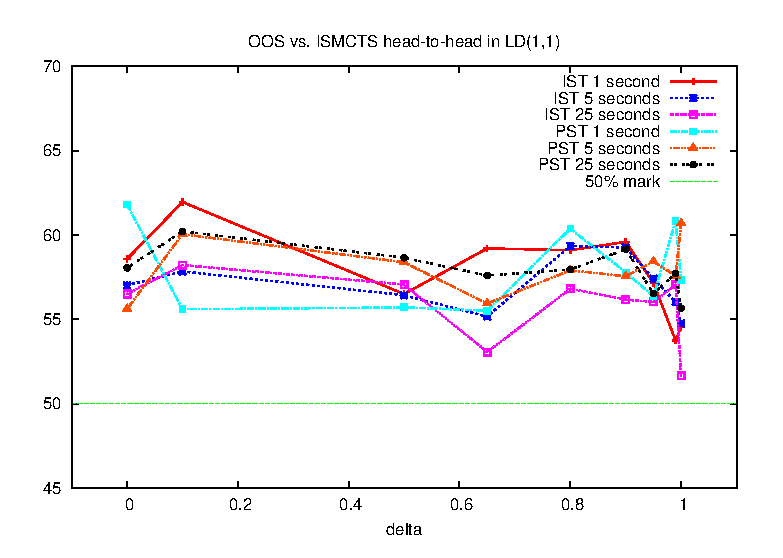
\includegraphics[scale=0.5]{plots/ismcts-oos-perf} \\
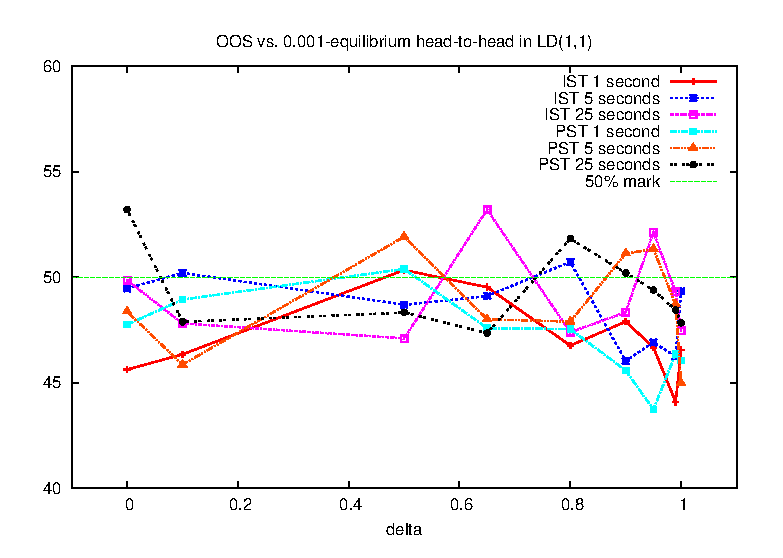
\includegraphics[scale=0.5]{plots/eq-oos-perf} \\
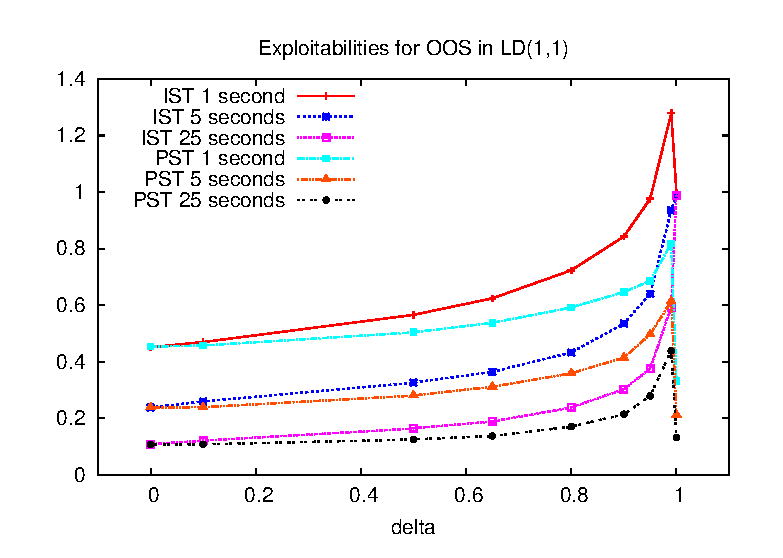
\includegraphics[scale=0.5]{plots/oos-expl} \\
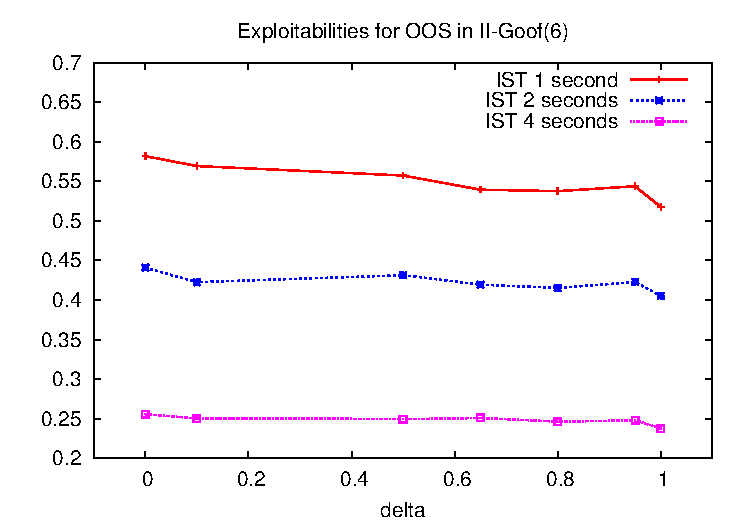
\includegraphics[scale=0.5]{plots/goof-expl} \\
\caption{Results for OOS in LD(1,1). From top: win rate (\%) of OOS vs. ISMCTS, win rate (\%) of 
OOS vs. a 0.001-equilibrium, approximate $\epsilon_{\sigma}$ using aggregate method in LD(1,1) 
and II-Goofpiel(6).}
\label{fig:results}
\end{center}
\end{figure}


In our experiments ISMCTS uses $C = 2$; tuning shows that the $C$ value does not 
affect the performance. 
In II-Goofspiel(6) we run searches for 1, 2, and 4 seconds.
As there are no public actions, we only compare IST in II-Goofspiel. 
Over a range of values for $\delta$ and all time settings, there was no statistically significant
winner in head-to-head matches between IST and ISMCTS. 
Exploitability is shown in Figure~\ref{fig:results}. We observe that exploitability generally 
decreases as search time increases and also as $\delta$ increases, with its lowest points at $\delta = 1$. 
The positive result was surprising, and we suspect it is due to benefiting from the reuse of 
values from previous searches from the same match.

In LD(1,1), we try searches for 1, 5, and 25 seconds. 
Among all values for delta and time settings, IST wins 79.2-86.7\% and PST wins 78.6-84.0\%, with a 
non-noticeable difference over different $\delta$ values. 
In LD(1,1) when played against a uniform random player ISMCTS wins 79.8-82.4\% at 1, 5, and 25 seconds. 
Upon further inspection, ISMCTS very quickly converges to the same strategy every time: as first player, 
with a weak roll ($r = \epsdice{1}, \epsdice{2},$ or \epsdice{3}) it bids 2-$r$ in the hope that by chance the
opponent has the same roll because if it did not, the second player would have a winning response most of the time.
On a roll of $r = \epsdice{4}$ or $r = \epsdice{5}$ it always bids 1-$r$ because it wins most of time. Either way, as 
second player ISMCTS selects responses based on the same reasoning, inducing the first player's roll based on their
first bid. This also explains the relative exploitability values in Table~\ref{tbl:fullstitching}: the first player
plays overly safely and hence is hard to exploit, meanwhile the second player best-responds to an expected pure first 
player strategy, which makes it highly exploitable. 
Our exploitability experiments shows a similar skewed first vs. second player effect in II-Goofspiel. 

Results OOS variants on LD(1,1) are shown in Figure~\ref{fig:results}. Firstly, in head-to-head performance 
we notice OOS wins 55-60\% of games against ISMCTS, results for $\delta \in \{ 0.1, 0.8, 0.9 \}$ seem somewhat 
consistent across variants and time settings, with varied effects for $\delta > 0.9$. 
Against the 0.001-equilibrium strategy, 
$\delta = 0.5, 0.65$ seems the most robust across variants and time settings, with varied effects when $\delta > 0.9$.
There are some clear trends for the exploitability of OOS strategies. First, exploitability of the global strategy 
increases with $\delta$, and again $\delta = 1$ gives surprisingly good results. 
The sudden drop could be caused by the fact that when $\delta = 0.99$, the 
importance of the off-match samples are weighted heavily which compete with the targeted samples. 
PST is less affected than IST by the targeting and appears to have lower exploitability. 
For each method and all values of $\delta$: increasing the search time decreases exploitability. 
The exploitability values from Table~\ref{tbl:fullstitching} also show this trend, and exploitability values of 
ISMCTS show locked in at at $\approx$ 0.8, which we have also confirmed via the aggregate method.

We performed one head-to-head experiment consisting of 500 games of PST($\delta = 0.8$) vs. ISMCTS, in LD(2,2)
with 25 seconds of search time. 
PST won 256 games, showing a competitive promise on 
this much larger game with roughly 352 million information sets. 

Finally, inspired by~\cite{Auger11Multiple}, we started an initial investigation of OOS and ISMCTS in Phantom Tic-Tac-Toe. 
We noticed that the mixed distribution obtained by normalizing the visit counts of ISMCTS was producing a 
similar distribution at the root as OOS. As in the Rock, Paper, Scissors example~\cite{Shafiei09}, 
we designed a biased version that gave higher payoff if the final line included a side. This 
led to OOS and ISMCTS producing two distinctly different distributions at the root. 

\begin{table}
{\small
\begin{center}
\begin{tabular}{ccccc}
Algorithm     & Time & $\epsilon_1$ & $\epsilon_2$ & $\epsilon_\sigma$ \\
\hline
ISMCTS        & 1s   & 0.235  & 0.574  & 0.808 \\
IST           & 1s   & 0.337  & 0.311  & 0.648 \\
PST           & 1s   & 0.203  & 0.211  & 0.414 \\
\hline
ISMCTS        & 5s   & 0.251  & 0.548  & 0.799 \\
IST           & 5s   & 0.229  & 0.295  & 0.524 \\
PST           & 5s   & 0.148  & 0.125  & 0.273 \\
\hline
\end{tabular}
\caption{LD(1,1) exploitability using full-stitching, $\delta = 0.9$.} 
\label{tbl:fullstitching}
\end{center}
}
\end{table}


\section{Conclusion}

In the paper, we have introduced Online Outcome Sampling, the first 
imperfect information search algorithm that is guaranteed to produce 
approximate equilibrium strategies as search time is increased. We 
showed that in head-to-head performance, OOS is able to compete with 
ISMCTS while producing strategies with lower exploitability
at the same search time in Liar's Dice and II-Goofspiel.

For future work, we hope to derive finite-time convergence guarantees 
and apply OOS to larger games such as no-limit Poker. 
We also plan to try MCRNR~\cite{Ponsen11Computing} instead of MCCFR 
to balance exploitability and exploitation versus known opponents.

\bibliographystyle{aaai}
\bibliography{iioos}

\end{document}
